%
%  PARA TRABALLOS EN GALLEGO USAR (LINEA 12): \usepackage[galician]{babel}
%  PARA TRABALLOS EN CASTELLANO USAR (LINEA 13): \usepackage[spanish]{babel}
%
% Para los acentos usamos codificacion UTF-8 (LINEA 10): \usepackage[utf8]{inputenc} 
% Si se usase la codificacion es_ES.ISO-8859-1 (LINEA 11): \usepackage[latin1]{inputenc}
% La conversion de acentos se hace con: iconv -f UTF-8 -t ISO-8859-1 filename.tex
%
% Como se incluyen figuras eps hay que compilar con: latex traballo , dvipdf traballo
%

\documentclass[12pt,twoside,a4paper]{book}
% pódense engadir todos os packages necesarios
\usepackage[utf8]{inputenc}
% \usepackage[latin1]{inputenc}
\usepackage[galician]{babel}
% \usepackage[spanish]{babel}
\usepackage{graphicx}
\usepackage[dvips]{epsfig}
\usepackage{amssymb}
\usepackage{eurosym}
\usepackage{float}
\usepackage{latexsym}
\usepackage{a4}
\usepackage{listings}
% \usepackage{hyperref} % menús no pdf pero non leva ben co package galician


\addto\captionsgalician{\def\contentsname{Memoria tipo B -- \'{I}ndice xeral }}
	

\begin{document}
\pagestyle{empty}
\begin{center}
	{\bf\Large UNIVERSIDADE DE SANTIAGO DE COMPOSTELA}
	
	\vspace{0.5cm}
	
\includegraphics[width=5cm]{figuras/logo_usc.eps}
	
	\vspace{0.5cm}
	{\bf\large ESCOLA TÉCNICA SUPERIOR DE ENXEÑARÍA}
	
	\vspace{3cm}
	{\bf\LARGE Seguimento de contaminación de cidades españolas a partir de datos de TROPOMI}
	
	%\vspace{0.5cm}
	%{\bf\LARGE Subtítulo do Traballo de Fin de Grao}
\end{center}

\vspace{2cm}
\hspace{4cm}\begin{tabular}{l}
	{\it\Large Autor/a:} \\
	{\bf\Large Hugo Gómez Sabucedo} \\
	~ \\
	{\it\Large Titores:} \\
	{\bf\Large Joaquín Ángel Triñanes Fernández} \\
\end{tabular}

\vspace{2cm}
\begin{center}
	{\bf\Large Grao en Enxeñaría Informática}
	
	\vspace{0.5cm}
	{\bf\large Febreiro 2024}
	
	\vspace{0.5cm}
	Traballo de Fin de Grao presentado na Escola Técnica Superior de Enxeñaría da Universidade de Santiago de Compostela para a obtención do Grao en Enxeñaría Informática
\end{center}


\cleardoublepage
\pagestyle{plain}
\pagenumbering{roman}

\includegraphics[width=4cm]{figuras/logo_usc.eps}

\vspace{1cm}
{\bf D. Joaquín Ángel Triñanes Fernández}, Profesor/a do Departamento de Electrónica e Computación da Universidade de Santiago de Compostela,

\vspace{1cm}
INFORMA:

\vspace{1cm}
Que a presente memoria, titulada {\it (Seguimento de contaminación decidades españolas a partir de datos de TROPOMI)}, presentada por {\bf D. Hugo Gómez Sabucedo} para superar os créditos correspondentes ao Traballo de Fin de Grao da titulación de Grao en Enxeñaría Informática, realizouse baixo nosa titoría no Departamento de Electrónica e Computación da Universidade de Santiago de Compostela.

\vspace{1cm}
E para que así conste aos efectos oportunos, expiden o presente informe en Santiago de Compostela, a (Data):

\vspace{2cm}
\begin{tabular}{lll}
	Titor/a, & Alumno/a, \\
	~ \\
	~ \\
	~ \\
	~ \\
	~ \\
	~ \\
	~ \\
	(Joaquín Ángel Triñanes Fernández) & (Hugo Gómez Sabucedo)
\end{tabular}

 % paxina de certificación (optativa)
\cleardoublepage
\pagestyle{plain}
\chapter*{Agradecementos}
Quero dar as grazas, en primeiro lugar, á miña familia, por apoiarme sempre ó longo de tódolos meus estudos. Sen o voso apoio e o voso amor, nada disto sería posible.

Tamén quero agradecer ós meus amigos, ós que estaban e ós que viñeron. Grazas por estar sempre aí, polo apoio e por servir de distración, moitas veces, nos momentos malos.

 % paxina de agradecementos (optativa) 
\cleardoublepage
\pagestyle{plain}
\chapter*{Resumo}
A presenza de diferentes axentes contaminantes na atmosfera é a causa non só do cambio climático, senón de moitos problemas de saúde para as persoas. Actualmente, dispoñemos de múltiples satélites
que nos permiten monitorizar os niveis destes parámetros de forma remota. Porén, analizar multitude de arquivos e datos, para diversos parámetros e días, pode ser unha tarefa tediosa.

É por iso que se propón este traballo, que ten como obxectivo deseñar un sistema para monitorizar a variabilidade e tendencia de diferentes parámetros obtidos a través de datos de satélite.
Mediante a descarga destes datos e a súa transformación e agregación, poderemos reducir significativamente a cantidade de arquivos que será preciso analizar, o cal facilita o seguimento da
contaminación por parte dos usuarios finais. O desenvolvemento deste sistema farase de forma que se poida acceder a el facilmente, e tendo en conta tamén a interoperabilidade do mesmo. % páxina de resumo (optativa) 

\cleardoublepage
\pagestyle{plain}
\tableofcontents
\listoffigures
\listoftables

% Agora incluimos os capítulos. Cambiamos a numeración e as cabeceiras
\cleardoublepage
\pagenumbering{arabic}
\setcounter{page}{1}
\pagestyle{headings}
\chapter{Introdución}\label{introducion}
\hyphenation{In-te-re-se}

O cambio climático é un asunto que, actualmente, está á orde do día. O aumento das temperaturas a nivel global é un asunto que preocupa non só ós
científicos, senón tamén á poboación en xeral. As causas do cambio climático son moitas, pero podemos estar de acordo en que unha gran parte é
debida á presenza de múltiples gases ou substancias químicas que afectan á atmosfera.

A presenza destes axentes contaminantes tamén afecta en gran medida ós seres humanos. Moitas enfermidades presentes na sociedade de hoxe en día son debidas
a un exceso de contaminación atmosférica. Doenzas respiratorias, coma a asma, ou alerxias son problema de saúde que están cada vez máis presentes, e que afectan
negativamente á calidade de vida das persoas.

Por iso, monitorizar a evolución destes axentes é algo crucial, sobre todo en entornos especialmente críticos, como poden ser as cidades, nas cales a conxunción
dunha gran densidade de poboación e de movementos en áreas, polo xeral, pequenas, fai que sexa crucial coñecer cal é o nivel destes axentes. Desta forma, as
autoridades poden adoptar medidas, tanto de saúde pública (como poden ser plans de prevencións de diferentes enfermidades), coma de proteción do medio ambiente
(limitando, por exemplo, a circulación de vehículos), co obxectivo de evitar que se causen danos ó entorno en que vivimos e reducir a mortalidade debida a
estas enfermidades.

Así, dende a Axencia Espacial Europea (ESA) lanzouse, no ano 2017, un satélite de observación terreste nomeado Sentinel-5 Precursor (ou Sentinel-5P).
Dito satélite, que se enmarca dentro do Programa COPERNICUS, emprega un instrumento denominado espectrómetro, co obxectivo de monitorizar a contaminación
atmosférica. Desta forma, TROPOMI proporciona observacións de forma diaria de gases atmosféricos que son chave á hora de monitorizar a calidade do aire
e realizar predicións sobre a evolución da mesma, coma poden ser o metano ($CH_{4}$), monóxido de carbono ($CO$), formaldehído ($HCHO$), dióxido de nitróxeno
($NO_{2}$), ozono ($O_{3}$), aerosol ou dióxido de xofre ($SO_{2}$).

Este satélite proporciona datos a dous niveis distintos: L1, con datos crus; e L2, con variables xeofísicas derivadas dos datos de nivel 1. Existe outro nivel,
o Nivel 3 (L3), no cal as variables están mapeadas en escalas regulares. Será este o nivel que nos interese alcanzar nos nosos datos, para poder obter con eles
un agregado mensual que nos permita ver a media ou crear climatoloxías para poder observar anomalías nos mesmos.

O obxectivo deste traballo é, por tanto, empregar os datos que nos proporciona este satélite para, mediante a realización de diferentes operacións sobre
os mesmos, poder facer un seguimento da evolución ó longo do tempo da contaminación en diversas cidades de España. Decidiuse escoller este ámbito debido
a que, ó tratarse dun área relativamente reducida, o procesamento dos datos será máis sinxelo, posto que será preciso procesar menos arquivos de menor tamaño.


\section{Obxectivos do traballo}\label{obxectivos}
Os obxectivos deste traballo de fin de grao son os seguintes:
\begin{enumerate}
    \item Mapear a contaminación atmosférica a partir de datos de sensores remotos, con especial relevancia en entornos urbanos
    \item Monitorizar a variabilidade e tendencia dos diferentes parámetros satelitais relacionados coa contaminación do aire.
    \item Desenvolver un visor online que permita representar de forma dinámica a información.
    \item Implementar un sistema interoperable de distribución dos datos e produtos.
\end{enumerate}

\section{Estrutura da memoria}\label{estrutura}
A presente memoria estrutúrase do seguinte xeito:
\begin{itemize}
    \item \textbf{Capítulo 2:} Especificación de requisitos. Este capítulo describe detalladamente os requisitos e criterios que debe cumprir o proxecto.
    \item \textbf{Capítulo 3:} Deseño. Aquí explicaremos todo o relativo ó proceso de deseño do software ata acadar a súa versión final. Tamén se comenta a
    metodoloxía empregada para o seu desenvolvemento, así como as diferentes tecnoloxías das que se fixo uso no mesmo.
    \item \textbf{Capítulo 4:} Probas. Esta sección trata sobre as probas realizadas, así como os resultados das mesmas.
    \item \textbf{Capítulo 5:} Conclusións e posibles ampliacións. Neste último capítulo preséntanse as conclusións obtidas após realizar o proxecto,
    así como propostas de melloras sobre o mesmo ou posibles ampliacións futuras.
\end{itemize}

\section{Descrición do sistema}\label{descricion}
Como se explicou nos \hyperref[sec:obxectivos]{obxectivos do traballo}, o sistema que deseñemos terá como finalidade poder monitorizar a variabilidade e tendencia
de diferentes parámetros, obtidos a través de datos de satélite, os cales se empregan para medir a contaminación do aire.

Será preciso, por tanto, deseñar un módulo  mediante o cal poidamos descargar os datos de TROPOMI, obtidos a través da ESA, para poder traballar con eles, realizando
as transformacións anteriormente mencionadas. Así, empregando as APIs proporcionadas, poderemos deseñar unha función que busque un determinado produto (por exemplo,
$NO_{2}$) no catálogo de COPERNICUS, filtrando os resultados para centrarnos nun área de interese (neste caso, a Península Ibérica) e datas concretas. Construíndo unha
query, e empregando a librería \texttt{requests}, descagaremos os arquivos para, posteriormente, transformalos. Ademais, os arquivos veñen en formato \texttt{.zip}, polo que será
preciso, neste módulo, descomprimilos para poder obter os arquivos de formato \texttt{.nc} cos que debemos traballar. Este módulo será desenvolvido na linguaxe Python.

Por outra parte, deseñaremos outro módulo, tamén en Python, no cal poidamos traballar cos arquivos descargados. Os datos que descargamos son de nivel 2, polo que temos que realizar
operacións cos mesmos para transformalos en datos agregados por mes. Para isto, será preciso empregar \texttt{HARP}, unha ferramenta que permite ler e procesar datos de satélite,
permitindo a inxesta de arquivos e o traballo cos mesmos. Así, importaremos tódolos arquivos descargados e realizaremos as transformacións anteriormente citadas, para posteriomente
exportar o resultado nun arquivo, tamén de formato \texttt{.nc}, nun directorio específico.

Os datos transformados almacenaranse nun servidor ERDDAP, que empregaremos como middleware. Este servidor proporciona unha forma sinxela de acceder a datasets científicos en formatos
de arquivos comúns, facilitando a xeración de gráficos e mapas. Unifica diferentes tipos de servidores con diferentes estruturas e devolve os datos nun formato de arquivo común, así
como estandariza as datas entre os mesmos. Ademais, é posible configurar un servidor ERDDAP propio e empregar os nosos propios datos. Esta será a opción que elixamos, xa que nos permite
empregar os datos que nós mesmos transformamos.

Será preciso establecer, no servidor onde corra a aplicación, unha tarefa automática, para que, segundo se publiquen datos novos, estes estean dispoñibles na nosa aplicación. Esta tarefa
deberá executarse tódolos meses, tendo en conta que os datos das medicións de satélite tardan uns días en estaren dispoñibles, e deberá descargar os datos dos parámetros que empregue a
nosa aplicación, transformalos e almacenalos no directorio establecido.

Por último, deseñaremos unha interface web que permitirá consultar a evolución de cada un dos diferentes parámetros (escollendo un deles) ó longo do tempo.

Todo isto implementarémolo nunha máquina de AWS, de forma que o sistema se administrará dende a mesma. Así, poderemos acceder á interface web de forma sinxela, a través de internet,
e toda a xestión da aplicación estará tamén centralizada. Nesta máquina almacenaremos os datos transformados que obteñamos do módulo de Python, e nela teremos tamén o servidor ERDDAP
co cal acceder a ditos datos. Accedendo á máquina poderemos visualizar a interface web que mencionamos.

\cleardoublepage
\chapter{Especificación de Requisitos}

Especificación dos requisitos máis relevantes do Sistema, xunto coa información que este debe almacenar e as interfaces
con outros Sistemas, sexan hardware ou software, e outros requisitos (rendemento, seguridade, etc.).

\cleardoublepage
\chapter{Deseño}

%Debe describirse como se realiza o Sistema, a división deste en diferentes compoñentes e a comunicación entre eles.
%Así mesmo, determinarase o equipamento hardware e software necesario, xustificando a súa elección no caso de que non fose
%un requisito previo. Debe achegarse a un nivel suficiente de detalle que permita comprender a totalidade da estrutura do
%produto desenvolvido, utilizando no posible representacións gráficas.
Neste capítulo, explicaremos  os diferentes compoñentes que forman o sistema e as tecnoloxías empregadas, así como o proceso de desenvolvemento e implementación do mesmo.

\section{Compoñentes do sistema}
No que respecta á arquitectura do sistema software desenvolvido, podemos identificar tres grandes compoñentes:
\begin{itemize}
    \item \textbf{Backend}

    \item \textbf{Middleware}

    \item \textbf{Frontend}

\end{itemize}

\section{Tecnoloxías empregadas}
\subsection{Anaconda}

\section{Desenvolvemento do sistema}

\section{Implementación do sistema}
\cleardoublepage
\chapter{Probas}

%Plan de probas (con evidencias) que verifica a funcionalidade e correctitude global do sistema, e se leva a cabo.


\cleardoublepage
\chapter{Exemplos (eliminar capítulo na versión final)}

\section{Un exemplo de sección}
Esta é {\it letra cursiva}, esta é {\bf letra negrilla}, esta é \underline{letra subrallada}, e esta é {\tt letra curier}. Letra {\tiny tiny}, {\scriptsize scriptsize}, {\small small}, {\large large}, {\Large Large}, {\LARGE LARGE} e moitas más. Exemplo de fórmula: $a=\int_o^\infty f(t)dt$.  E agora unha ecuación aparte:

\begin{equation}
S=\sum_{i=0}^{N-1} a_i^2 .
\label{mi_ecuacion}
\end{equation}

As ecuaciones se poden referenciar: ecuación (\ref{mi_ecuacion}).

\subsection{Un exemplo de subsección}
O texto vai aquí.
\subsection{Otro exemplo de subsección}
O texto vai aquí.
\subsubsection{Un exemplo de subsubsección}
O texto vai aquí.
\subsubsection{Un exemplo de subsubsección}
O texto vai aquí.
\subsubsection{Un exemplo de subsubsección}
O texto vai aquí.
\section{Exemplos de figuras e cadros}

A figura número \ref{enlace1}.

O cadro (taboa) número \ref{enlace2}.

\begin{figure}
\centerline{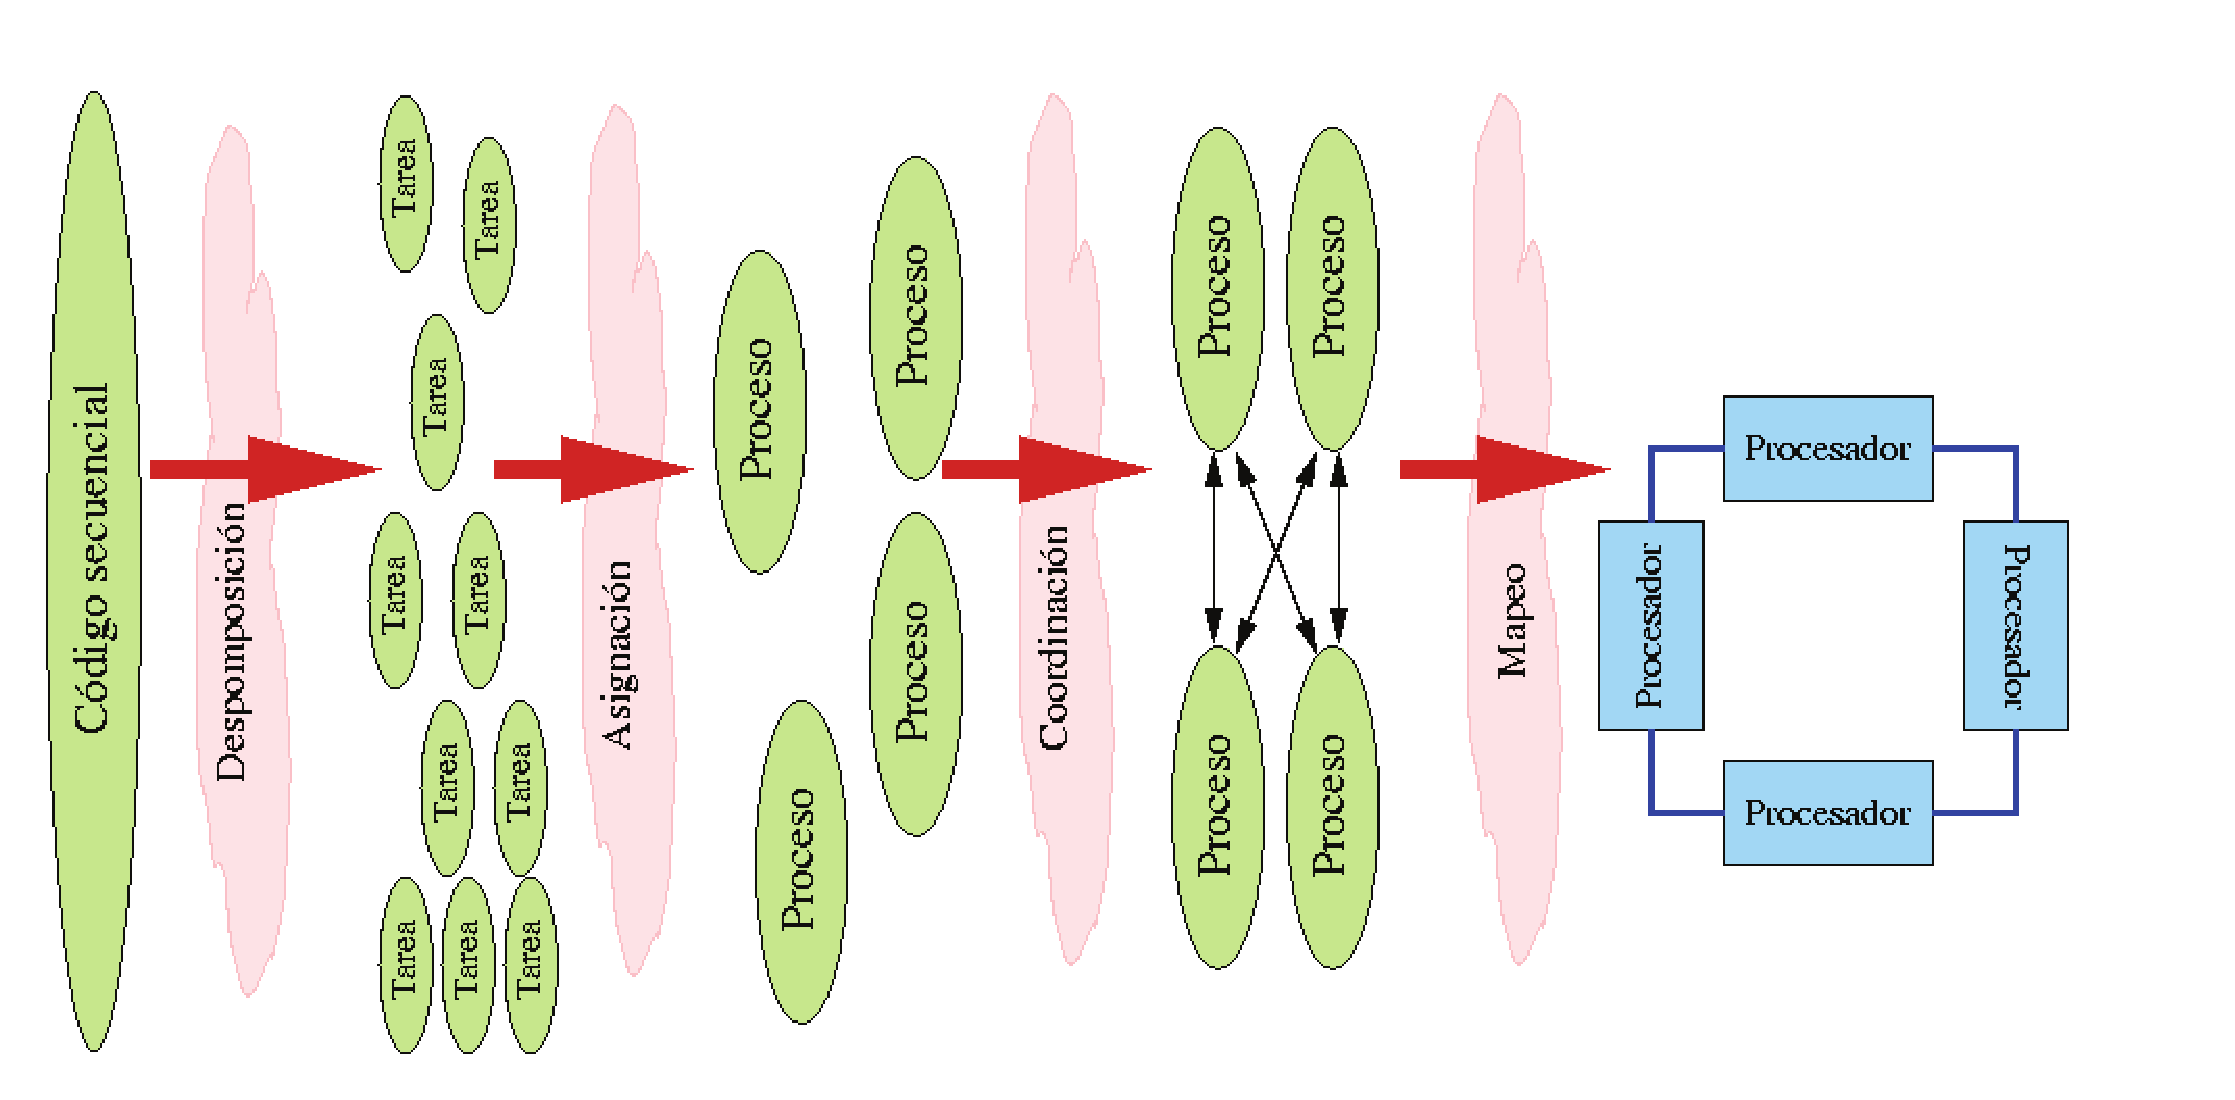
\includegraphics[width=15cm]{figuras/figura01.eps}}
\caption{Esta é a figura de tal e cal.}
\label{enlace1}
\end{figure}

\begin{table}
\begin{center}
\begin{tabular}{|l||r|c|} \hline
Izquierda & Derecha & Centrado  \\ \hline\hline
ll & r & cccc \\ \hline
llll & rrr & c \\ \hline
\end{tabular}
\caption{Esta é a táboa de tal e cal.}
\label{enlace2}
\end{center}
\end{table}

\section{Exemplos de referencias á bibliografía}
Este é un exemplo de referencia a un documento descargado da web \cite{cuda}. E este é un exemplo de referencia a unha páxina da wikipedia \cite{cdma}. Agora un libro \cite{gonzalez} e agora unha referencia a un artigo dunha revista \cite{patricia}. Tamén se poden pór varias referencias á vez \cite{cuda,gonzalez}.

\section{Exemplos de enumeracións}

Con puntos:

\begin{itemize}
\item Un.
\item Dous.
\item Tres.
\end{itemize}

Con números:

\begin{enumerate}
\item Catro.
\item Cinco.
\item Seis.
\end{enumerate}

Exemplo de texto verbatim:

\begin{verbatim}
O texto        verbatim 
     se visualiza tal
            como se escribe
\end{verbatim}

Exemplo de código C:

\lstset{language=C}

\begin{lstlisting}
#include <math.h>
main()
{  int i, j, a[10];
   for(i=0;i<=10;i++) a[i]=i; // comentario 1
   if(a[1]==0) j=1; /* comentario 2 */
   else j=2;
}
\end{lstlisting}

Exemplo de código Java:

\lstset{language=java}

\begin{lstlisting}
class HelloWorldApp {
    public static void main(String[] args) {
        System.out.println("Hello World!"); // Display the string.
    }
}
\end{lstlisting}



%
% Engadir os capitulos que fagan falta
%
\cleardoublepage
\chapter{Conclusións e posibles ampliacións}
O obxectivo principal deste traballo era deseñar un sistema para a monitorización da variabilidade e tendencia de diferentes parámetros empregados para medir a contaminación do aire, con datos
obtidos mediante medicións de satélite. Así, buscábase aproveitar os datos dispoñibles na web de COPERNICUS para traballar con eles, creando agregados mensuais, de forma que os usuarios os puideran
empregar para seguir a evolución da contaminación atmosférica.

Este sistema ofrece a posibilidade de consultar, para a Península Ibérica, os valores de catro parámetros diferentes ó longo do ano 2023. Estes parámetros son o monóxido de carbono ($CO$), o ozono
($O_3$), o dióxido de nitróxeno ($NO_2$) e o dióxido de xofre ($SO_2$). Mediante unha interface sinxela, podemos visualizar nun mapa o valor destes parámetros, que se mapearon a unha cuadrícula
regular que abarca toda a área de interese.

O usuario ten, desta forma, fácil acceso ós datos de satélite, podendo visualizar os mesmos dunha forma sinxela. Posto que os arquivos individuais de cada un dos parámetros teñen un gran tamaño,
mediante a agregación dos mesmos de forma mensual podemos reducir drasticamente as necesidades de almacenamento, o cal resulta realmente beneficioso tendo en conta que, para un ano, poderiamos
estar falando de cantidades en torno a 300GB de datos para cada parámetro por ano, mentres que o noso sistema precisa menos de 1GB por parámetro.

Desta forma, podemos considerar que se satisfixeron os catro obxectivos que se definiron en \ref{obxectivos}. Logrouse mapear a contaminación atmosférica mediante os datos de sensores remotos,
mediante a transformación dos datos dispoñibles no dataspace COPERNICUS da ESA e a súa transformación a nivel L3. Conseguimos monitorizar a variabilidade e tendencia dos parámetros relacionados coa
contaminación do aire, tanto de forma xeográfica, visualizándoos nun mapa, como a través de gráficos de liñas. En relación con isto, tamén desenvolvimos un sinxelo visor online, para representar a
información de forma gráfica e dinámica. Por último, implementouse un sistema interoperable para distribuír os datos, posto que o propio servidor ERDDAP permite compartir e distribuír os datos con
outros sistemas, dunha forma uniforme.

Para rematar, propóñense unha serie de melloras que se poderían aplicar ó sistema para facelo máis completo e adaptable ás necesidades dos usuarios:
\begin{enumerate}
    \item \textbf{Maior dispoñibilidade de datos}. Os parámetros dispoñibles no dataspace de COPERNICUS inclúen, ademais dos analizados neste traballo, o metano ($CH_4$), formaldehído ($HCHO$), a
    fracción de nubes ou o índice UV. Estes parámetros tiveron que descartarse do proxecto por falta de tempo, polo que podería ser interesante incluílos en ampliacións futuras. Asimesmo, os datos
    están dispoñibles dende mediados do ano 2018, polo que tamén sería factible ampliar a dispoñibilidade temporal dos mesmos, que actualmente é dende xaneiro de 2023 ó presente. Tamén se podería
    ampliar a área de análise dos datos a todo o continente europeo, ou incluso a todo o mundo.
    \item \textbf{Capacidade de automatización}. Podería ser útil integrar utilidades de automatización no sistema, de forma que os usuarios puideran recibir, de forma automática, algúns gráficos
    que eles mesmos elixan segundo teñamos novos produtos dispoñibles, para facilitármoslles a análise dos mesmos.
    \item \textbf{Mellora da experiencia e interface de usuario}. Unha forma de mellora da interface de usuario sería crear unha interface de JavaScript empregando leaflet. Isto non puido levarse a
    cabo neste proxecto, pero podería ser práctico en caso de aumentar tamén a dispoñibilidade de datos, xa que nos permite unha maior interacción cos mapas. Tamén poderían implementarse
    visualizacións en forma de gráficos 3D.
    \item \textbf{Creación dun \textit{dashboard} para visualizar os parámetros en distintas zonas da Península}. Proponse a creación dun taboleiro que permita, a partir dos datos dos que se dispón,
    centrarse en diferentes áreas urbanas da Península (por exemplo, a área metropolitana de Madrid ou a de Barcelona), para analizar máis en profundidade o valor e a evolución dos diferentes par
    ámetros. Tamén se podería introducir, neste taboleiro, un apartado mediante o cal visualizar as zonas quentes; é dicir, aquelas zonas con valores especialmente altos de diferentes parámetros
    nun mes en concreto, ou de forma prolongada no tempo.
    \item \textbf{Integración con Machine Learning}. Como un campo que está actualmente en auxe, o machine learning resulta especialmente relevante no ámbito da monitorización ambiental, xa que nos
    permitiría, a partir dos datos dos que dispoñemos, identificar patróns nos mesmos co obxectivo de elaborar predicións. Desta forma, poderíamos crear, por exemplo, agregacións semanais no canto
    de mensuais, o que nos permitiría dispoñer de información máis pormenorizada e realizar mellores análises. Isto podería empregars en colaboración con diferentes cidades, para saberen cando
    activar, por exemplo, os seus plans anticontaminación.
    \item \textbf{Análises estatísticos}. Por último, proponse a incorporación de ferramentas estatísticas para mellorar a experiencia dos usuarios á hora de analizar os datos. Por exemplo, poder
    ían implemantarse algoritmos para a detección de anomalías, ou para realizar directamente análises temporais e seguementos dos cambios dos diferentes parámetros ó longo do tempo.
\end{enumerate}


% Aquí empezan os apéndices
\appendix
\cleardoublepage
\chapter{Manuais técnicos}\label{manuais}

%En función do tipo de Traballo e metodoloxía empregada, o contido poderase dividir en varios documentos. En todo caso,
%neles incluirase toda a información precisa para aquelas persoas que se vaian encargar do desenvolvemento e/ou modificación
%do Sistema (por exemplo código fonte, recursos necesarios, operacións necesarias para modificacións e probas, posibles
%problemas, etc.). O código fonte poderase entregar en soporte informático en formatos PDF ou postscript.
Este manual técnico explica como realizar a instalación do sistema e o seu mantemento por parte dos administradores.
\section{Instalación}\label{instalacion}
No repositorio de GitHub \url{https://github.com/hugogs02/TROPOMIVisor} dispoñemos de todo o código fonte da aplicación, tanto do backend de Python, coma da interface e os arquivos de configuración do
servidor ERDDAP. É preciso recalcar que, no caso de querer instalar o sistema no ordenador propio, este deberá empregar o sistema operativo Ubuntu. Para a súa instalación, é preciso seguir os
seguintes pasos:
\begin{enumerate}
    \item \textbf{Instalar Python}. O sistema require \textbf{Python 3.11.6}, o cal se instalará mediante Anaconda, para facilitar tamén a xestión e instalación de paquetes. Para instalar Anaconda
    , debemos descargar o instalador dispoñible en \url{https://www.anaconda.com/download#downloads} . Deberase dar permiso de execución (\texttt{chmod o+rx [filename]}). Será necesario seguir os
    pasos que indica o instalador, entre os que se inclúen elixir o directorio de instalación, engadilo ó PATH e inicializar a instalación co comando \texttt{conda init}. A continuación, 
    instalaremos os seguintes paquetes:
    \begin{itemize}
        \item calendar (vén preinstalado con Python).
        \item datetime (versión 5.4).
        \item dateutil.parser (versión 2.8.2).
        \item glob2 (versión 0.7).
        \item harp (versión 1.17). Instalado con conda-forge.
        \item os (vén preinstalado con Python).
        \item pandas (versión 2.1.4).
        \item requests (versión 2.31.0).
        \item shutil (vén preinstalado con Python).
        \item sys (vén preinstalado con Python).
        \item time (vén preinstalado con Python).
        \item zipfile36 (versión 0.1.3).
    \end{itemize}
    \item \textbf{Instalar Java}. A instalación de Java debe ser da versión 17 (ou superior). Instalar Java en Ubuntu é sinxelo, simplemente se debe executar o comando \texttt{apt install openjdk-17-jdk
    openjdk-17-jre} .
    \item \textbf{Configurar Tomcat}. Para configurar correctamente tomcat, débese crear un usuario tomcat (con \texttt{sudo useradd -m -d /opt/tomcat -U -s /bin/false tomcat}), e descargar o
    arquivo de Tomcat (versión 10) dende \url{https://tomcat.apache.org/download-10.cgi} . Este deberá ser descomprimido no directorio \textit{opt/tomcat} Accederase ó arquivo \texttt{/opt/tomcat/conf/tomcat-users.xml}
    para configurar os usuarios Manager e Host Manager. A continuación, crearase un servizo para Tomcat, mediante o comando \texttt{sudo nano \break/etc/systemd/system/tomcat.service}, engadindo as
    seguintes liñas:
    \begin{lstlisting}
    [Unit]
    Description=Tomcat
    After=network.target

    [Service]
    Type=forking

    User=tomcat
    Group=tomcat

    Environment="JAVA_HOME=/usr/lib/jvm/java-1.11.0-openjdk-amd64"
    Environment="JAVA_OPTS=-Djava.security.egd=file:///dev/urandom"
    Environment="CATALINA_BASE=/opt/tomcat"
    Environment="CATALINA_HOME=/opt/tomcat"
    Environment="CATALINA_PID=/opt/tomcat/temp/tomcat.pid"
    Environment="CATALINA_OPTS=-Xms512M -Xmx1024M -server -XX:+UseParallelGC"

    ExecStart=/opt/tomcat/bin/startup.sh
    ExecStop=/opt/tomcat/bin/shutdown.sh

    RestartSec=10
    Restart=always

    [Install]
    WantedBy=multi-user.target
    \end{lstlisting}
    A continuación, recargarase o \textit{systemctl} con \texttt{sudo systemctl daemon-reload} e arrancarase o servizo de Tomcat con \texttt{sudo systemctl start tomcat}. Configurarase Tomcat para
    que arranque co sistema, mediante o comando \texttt{sudo systemctl enable tomcat}. Por último, executarase \texttt{sudo ufw allow 8080} para permitir tráfico polo porto 8080.
    \item \textbf{Executar os scripts de Python para obtención de datos}. Empregando git, podemos descagar o código dispoñible no repositorio que indicamos anteriormente. Co código descargado, 
    podemos executar o script principal para descargar os datos. O formato de execución será: \texttt{python app.py produto data\_inicio data\_fin ruta\_descarga ruta\_procesado}. "produto" deberá
    ser un entre os dispoñibles (L2\_\_CO\_\_\_\_, L2\_\_NO2\_\_\_, L2\_\_O3\_\_\_\_, L2\_\_SO2\_\_\_), e a data deberá ter o formato AAAA-MM-DD
    \item \textbf{Configurar o servidor ERDDAP}. Para configurar o servidor ERDDAP, deberemos seguir as instrucións de \url{https://coastwatch.pfeg.noaa.gov/erddap/download/setup.html}, empregando
    os arquivos de setup.xml e datasets.xml que se descargaron do repositorio de GitHub.
    \item \textbf{Configurar a interface web}. Para a interface web, crearase unha aplicación nova de Tomcat. Isto farase creando unha nova carpeta no directorio \textit{/opt/tomcat/webapps/}, e
    copiando á mesma o arquivo HTML que se descargou do repositorio.
\end{enumerate}

Unha vez seguidos todos estes pasos, o sistema estará listo para o seu uso.

\section{Mantemento}\label{mantemento}
O mantemento do sistema é sinxelo, pois o administrador só precisa consultar o log de erros o día que se indicou no \textit{job} de cron para executar a actualización dos datos, e comprobar que
funcionou correctamente. En caso de que se rexistre algunha mensaxe de erro relativa á descarga dos arquivos, se esta se dá nun ou dous deles, pode ignorarse, posto que non afectara ó resultado. En
caso de que se produzan máis erros, será preciso executar o script principal manualmente, para realizar a descarga de datos. O mesmo será preciso en caso de ter algún erro coa importación e
transformación dos datos.

Tamén poden ocurrir erros ou problemas co servidor ERDDAP. Neste caso, o mellor é reiniciar Tomcat, empregando para iso os scripts \texttt{shutdown.sh} e \texttt{startup.sh}, ubicados en
\textit{/opt/tomcat/bin/} .
\cleardoublepage
\chapter{Manuais de usuario}

%Incluirán toda a información precisa para aquelas persoas que utilicen o Sistema: instalación, utilización, configuración,
%mensaxes de erro, etc. A documentación do usuario debe ser autocontida, é dicir, para o seu entendemento o usuario final
%non debe precisar da lectura doutro manual técnico.
O manual de usuario proporciona a información necesaria para o usuario final que desexa empregar o sistema de forma autónoma; é dicir, que o usuario non precise ler outro manual para empregar a
aplicación.

Para acceder á aplicación, o usuario debe acceder á seguinte URL: \url{http://13.53.65.240:8080/TROPOMIVisor/} , podendo ver a interface da figura \ref{fig:interfaz}. Nela, preséntaselle un
desplegable para elixir o parámetro, entre os 4 que hai dispoñibles (CO, SO2, NO2 ou O3); e un calendario dende o que pode elixir o mes do que quere consultar os datos. Ó realizar un cambio en
calquera destes dous parámetros, actualizarase automaticamente o mapa, amosándose o gráfico correspondente. O usuario deberá ter en conta o rango de datas dispoñible para consultar os datos, que
neste traballo é a partir de xaneiro de 2023. Ademais, deberá ter en conta que os datos do mes anterior (por exemplo, de xaneiro de 2024) non estarán dispoñibles ata aproximadamente o día 11 do
seguinte mes (neste caso, o 11 de febreiro), debido á latencia á hora de procesar os datos tanto no servidor local como por parte de COPERNICUS. Se intenta visualizar o mapa para un mes no que non
hai datos, a imaxe mostrará unha mensaxe de erro.

\begin{figure}
    \centerline{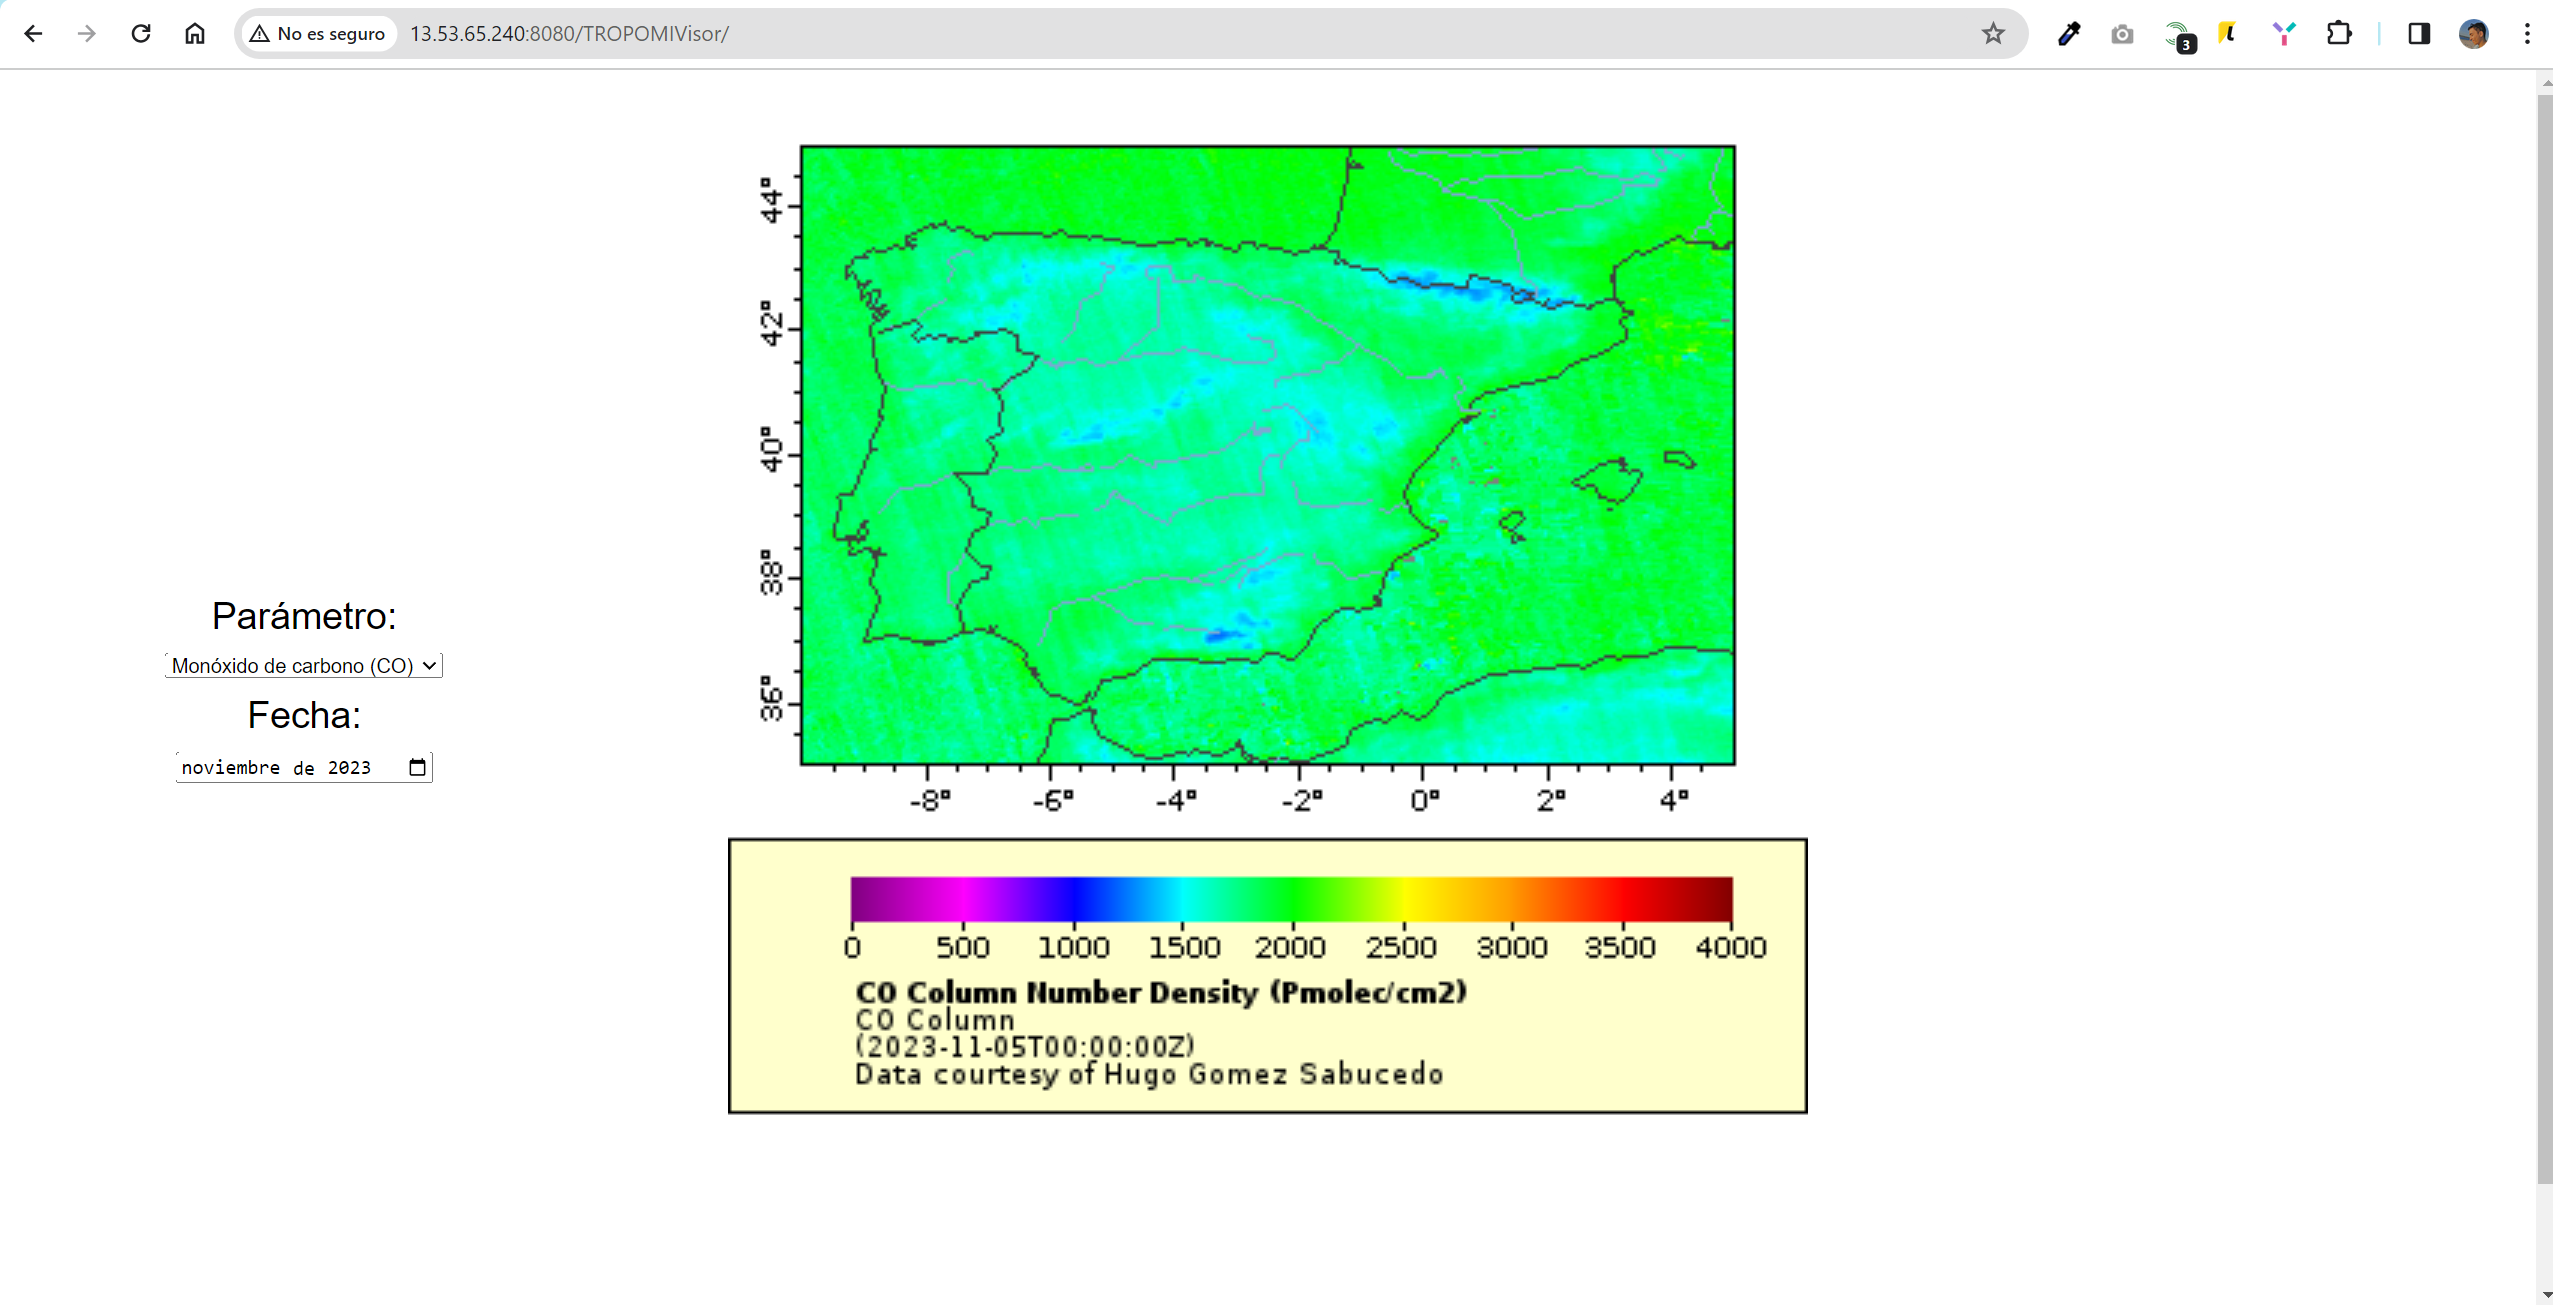
\includegraphics[width=10cm]{figuras/interfaz.png}}
    \caption{Exemplo da interface que se mostra ó acceder á aplicación.}
    \label{fig:interfaz}
\end{figure}

\cleardoublepage
\chapter{Licenza}
Se se quere pór unha licenza (GNU GPL, Creative Commons, etc), o texto da licenza vai aquí.


\cleardoublepage
\markboth{BIBLIOGRAFÍA}{BIBLIOGRAFÍA}
\addcontentsline{toc}{chapter}{Bibliografía}


\begin{thebibliography}{99}
% EXEMPLO DE DOCUMENTO DESCARGADO DA WEB
\bibitem{cuda} Nvidia CUDA programming guide. Versión 2.0, 2010. Dispoñible en {\it http://www.nvidia.com}.

% EXEMPLO DE PÁXINA DA WIKIPEDIA
\bibitem{cdma} Acceso múltiple por división de código. Artigo da wikipedia ({\it http://es.wikipedia.org}). Consultado o 2 de xaneiro do 2010.

% EXEMEPLO DE LIBRO
\bibitem{gonzalez} R.C. Gonzalez e R.E. Woods, {\it Digital image processing}, 3ª edición, Prentice Hall, New York, 2007.

% EXEMPLO DE ARTIGO DE REVISTA
\bibitem{patricia} P. González, J.C. Cartex e T.F. Pelas, ``Parallel computation of wavelet transforms using the lifting scheme'', {\it Journal of Supercomputing}, vol. 18, no. 4, pp. 141-152, junio 2001.
\end{thebibliography}



\end{document}
